\documentclass[a4paper,12pt]{article}
% IC2S2 Extended Abstract Template
% version 1.1, last updated 2018-01-26
% This template works best with PDFLaTeX
\usepackage[utf8]{inputenc}
\usepackage[english]{babel}
\usepackage{graphics}
\usepackage{graphicx}
\usepackage{mathptmx}
\usepackage[usenames, dvipsnames]{color}
\usepackage[normal]{threeparttable}
\usepackage{float}

\newcommand{\beq}{\begin{eqnarray}}
\newcommand{\eeq}{\end{eqnarray}}
\newcommand{\+}{\phantom{-}}

%\usepackage{natbib}
%\bibliographystyle{ksfh_nat}
\bibliographystyle{plain}

%Pleasure ensure the ic2s2.sty file is in the same directory as your LaTeX document
%This package will set the margin, header, etc. as required for submission
\usepackage{ic2s2} 

%Directory containing your figure files (optional)
%\graphicspath{{images/}} 

%Please complete the following meta information
\title{Network Structure, Efficiency, and Performance in WikiProjects}
\shorttitle{Network Structure, Efficiency, and Performance in WikiProjects}
\keywords{peer-production, networks, collaboration, wikipedia, social learning}
\author{Anonymous}
\date{} %Leave blank for submission
\confdates{July 12--15, 2018}
\conflocation{Northwestern University's Kellogg School of Management, Evanston, IL.~USA}


\begin{document}

\maketitle

%Feel free to retitle this section and to use \section or \section* as you see fit
\section*{Extended Abstract}

Large-scale collaboration in the absence of top-down control is notoriously
difficult\cite{freeman_tyranny_1972},
yet the internet has enabled decentralized collaborations at a global scale.
Wikipedia is one of the most visible examples,
with millions of self-organized editors collaboratively producing
a high-quality encyclopedia \cite{giles_internet_2005}.
A better theoretical understanding of such projects is desirable,
in order to identify best-practices and inform the design of new projects.
We focus specifically on how the network structure formed
by editor interactions within a WikiProject relate to
two variables:
{\em efficiency} (how much is accomplished by a unit of work)
and {\em performance} (the best quality typically reached).
We confirm behaviors observed in numerical and small-scale lab studies
\cite{kearns_experiments_2012,golub_naive_2010,mason_propagation_2008},
such as an overall trade-off between performance and efficiency.
However, we find evidence that some variables correlate positively with both variables.

We focus on WikiProjects on the English-language Wikipedia.
WikiProjects are groups of related articles,
and form distinct communities, with distinct norms and processes.
One of the main roles of a WikiProject is to assess the quality of articles
within that project, which we use to quantify article progress.
We also rely ondesignations of featured article (FA) or good article (GA) status,
which are decided independently of WikiProject assessments.
We combine multiple data sets from the English-language Wikipedia.
For information about edit history, we used a publicly-available data set containing
metadata about all edits from July 12, 2006 to December 2, 2015.
To get the rating history of each article,
we used a custom script to scrape the daily logs produced by WP 1.0 Bot for
all unique WikiProjects (2279)
between May 4, 2006 and December 2, 2015.
Finally, we used a publicly-available log of page events (including rename events)
to reconstruct the unique identifier for each article title mentioned in
the rating history logs.

We define efficiency as the mean number of articles that reach a grade level,
divided by the number of edits since the previous grade level.
Let $T(W,G)$ be the set of article assessment transitions from below grade $G$
to grade $G$ or higher in project $W$.
Let $N(W,G)$ be the number of articles in project $W$ which ever transition
from below grade $G$ to grade $G$ (or higher).
Let $r(t)$ be the number of article revisions since its previous grade transition.
The grade $G$ efficiency is:
\begin{eqnarray}
E(W,G)
&=&
\left[
\frac{1}{
N(W,G)
}
\sum_{t \in T(W,G)} \frac{r(t)}{g(t)}
\right]^{-1},
\end{eqnarray}
where $g(t)$ (the number of grade levels crossed by transition $t$)
divides edits evenly when transitions span multipel grade levels.
Our performance measure $P(W)$ is defined simply as
the percentage of articles in project $W$ which have reached
good or featured status:
\begin{eqnarray}
P(W) &=& \frac{f(W) + g(W)}{n(W)},
\end{eqnarray}
where $f(W)$ and $g(W)$ are the numbered of featured and good articles respectively,
and $n(W)$ is the total number of articles.


For each WikiProject, we construct and analyze the coeditor network:
with editors being connected if they have edited at least one article in common.
These relationships represent possible flows of information.
We focus specifically on mean degree, degree skewness, and path length.
High-degree editors have more collaborators,
which can increase diversity and access to information at the possible
expense of higher coordination costs
\cite{hong_groups_2004,golub_naive_2010}.
Highly skewed degree distributions can amplify the biases of high-degree
editors while reducing the need for explicit coordination
\cite{kearns_experiments_2012}.
Networks with shorter path lengths allow information to travel more quickly
at the possible expense of less localized diversity
\cite{mason_propagation_2008,barkoczi_social_2016}.
The mean path length is computationally intensive,
so we employ stratified sampling,
choosing sample sizes such that the relative error is less than 10,
and exclude the 183 largest projects.

Our main findings (Figure \ref{fig:eff-perf}, Table \ref{tab:model}) are as follows.
Despite an overall performance/efficiency trade-off (r = -0.12, p $<$ 0.001),
Low-degree coeditor networks tend to have both higher performance and higher efficiency.
Short path lengths tend to be associated with higher performance, consistent with a conformity-based learning strategy.
Structural inequality (degree skewness) is associated with lower performance.

Our findings shed light on the importance of network structure for successful
collaboration at very large scales.
Our empirical results are strictly correlative, not causal,
and further work is necessary to determine causality.
However, the consistency of our findings with those in numerical simulations
and small-scale lab studies helps solidify a picture of the role of network
structure in collaboration.
The higher efficiency and performance observed for low-degree projects might
suggest benefits of collaborations of small closely-knit teams,
while the correlations between path length and performance might suggest
overlapping team membership in order to connect distant parts of the network.
And the correlation of low degree skewness with performance may suggest
benefits of decentralized team structure.
These findings might be informative for developing collaboration policies,
for designing interventions to recommend tasks based on how they will
influence network structure,
or for creating interventions which seek to encourage the behavioral norms most
effective for existing network structure.

%\section*{Acknowledgment(s)} %Optional

%\section*{References}
\bibliography{paper}

\section*{Figures and Tables}

\begin{figure}[H]
\centering
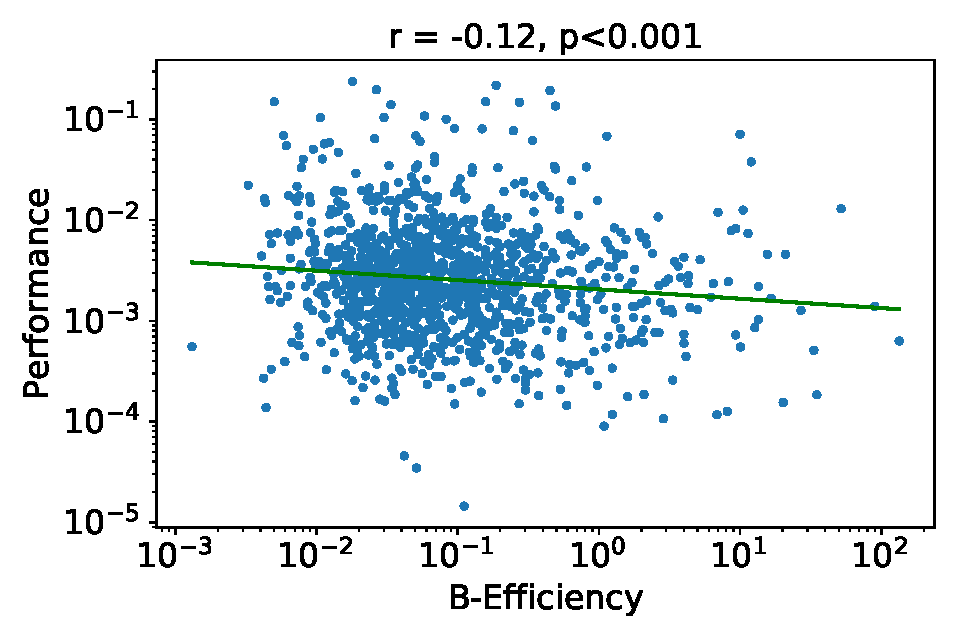
\includegraphics[width=4.5in,height=3in]{fig-perf-eff.pdf}
\caption{
WikiProject performance is anticorrelated with efficiency.
\label{fig:eff-perf}
}
\end{figure}

\begin{table}[H]
\centering
\small
\begin{tabular}{lllllllll}
&Perf$^\dagger$&A-Eff$^\dagger$&B-Eff$^\dagger$&C-Eff$^\dagger$\\
\hline
Mean degree$^\dagger$&-0.7$^{***}$&-0.8$^{***}$&-0.6$^{***}$&-0.3$^{*}$\\
Out degree skew$^\dagger$&-0.4$^{***}$&-0.5$^{**}$&-0.3$^{*}$&-0.06\\
Mean path length$^\dagger$&-0.33$^{***}$&-0.09&-0.05&-0.09\\
C-Efficiency$^\dagger$&-0.08$^{*}$&\+---&\+---&\+---\\
Connected frac.&0.01&0.09$^{*}$&0.15$^{***}$&0.06\\
Talk fraction$^\dagger$&0&-0.02&-0.03&0.01\\
Mean similarity$^\dagger$&0.06$^{**}$&-0.03&0.01&0.02\\
Mean editors/art.$^\dagger$&0.3$^{**}$&0.3&0.2$^{*}$&0.09\\
Article count$^\dagger$&-0.4&0.7$^{*}$&0.8$^{**}$&0.7$^{**}$\\
Editor count$^\dagger$&0.4&0.9$^{**}$&0.8$^{**}$&0.5$^{*}$\\
Revision count$^\dagger$&0.6$^{*}$&-1$^{**}$&-1.1$^{***}$&-1$^{***}$\\
First assessment&0.05&0.11$^{**}$&0.31$^{***}$&0.43$^{***}$\\
Mean article age&-0.03&-0.04&-0.01&-0.05$^{*}$\\
\hline
N&1179&966&1260&1415\\
R$^2_{adj}$&0.37&0.17&0.30&0.43\\
\hline
\end{tabular}
\begin{tablenotes}
\centering
\item $\dagger$ Log-transformed. * $p < 0.05$. ** $p < 0.01$. *** $p < 0.001$.
\end{tablenotes}
\caption{Standardized coefficients for OLS models.
\label{tab:model}
}
\end{table}

\end{document}
